An FFT algorithm computes the DFT of a signal in better than $\mathcal{O}(N^2)$ time. See Appendix \ref{theoryAppendix} for a review of the theory related to Fourier decomposition. 

The naive implementation of the DFT, as shown in section \ref{DFT_implementation}, has time complexity $\mathcal{O}(N^2)$. This can be done more efficiently with a divide and conquer approach. Consider the original equation for the DFT:
\[
X[k] = \sum_{n=0}^{N-1}x[n]e^{-i2\pi n k /N}
\]

Now split the sum in two, one with the even entries of $x[n]$ and one with odd:
\begin{align*}
X[k] &= \sum_{n=0}^{N-1}x[n]e^{-i2\pi n k /N}\\
&= \sum_{n=0}^{N/2-1}x[2n]e^{-i2\pi (2n) k /N} + \sum_{n=0}^{N/2-1}x[2n+1]e^{-i2\pi (2n+1) k /N}\\
&= \sum_{n=0}^{N/2-1}x[2n]e^{-i2\pi (2n) k /N} + e^{-i2\pi k/N}\sum_{n=0}^{N/2-1}x[2n+1]e^{-i2\pi (2n) k /N}\\
&= \sum_{n=0}^{N/2-1}x_e[n]e^{-i2\pi n k /(N/2)} + e^{-i2\pi k/N}\sum_{n=0}^{N/2-1}x_o[n]e^{-i2\pi n k /(N/2)}\\
&= X_e[k] + e^{-i2\pi k/N}X_o[k] \tag{*} \label{evenOdd} 
\end{align*}
where $x_e[n]$ and $x_o[n]$ are the signals formed by collecting the even and odd entries of $x[n]$, and $X_e[k]$ and $X_o[k]$ are the $N/2$ point DFTs of $x_e[n]$ and $x_o[n]$, respectively. This form of the DFT equation suggests that a divide and conquer strategy could be applied. We examine this now.

\subsection{Divide and Conquer DFT Complexity}
From an algorithmic perspective, the even-odd split of the DFT equation strongly suggests the use of recursion. What is the complexity in this case? Suppose the complexity of computing the DFT in this manner is given by $T(N)$, and that $N=2^{h}$, then
\begin{align*}
T(N) &= T(N/2) + T(N/2) + \mathcal{O}(N/2)\\
&= (T(N/4) + T(N/4) + \mathcal{O}(N/4)) \\
&\quad + (T(N/4) + T(N/4) + \mathcal{O}(N/4)) + \mathcal{O}(N/2)\\
&= 4T(N/4) + 2\mathcal{O}(N/4) + \mathcal{O}(N/2)\\
&= ...\\
&= 2^h T(1) + \sum_{i=1}^{h}2^i \mathcal{O}(N/2^i) \tag{**} \label{bottomOfTree}\\
&= N\mathcal{O}(1) + \sum_{i=1}^{\log N} \mathcal{O}(N)\\
&= \mathcal{O}(N) + \mathcal{O}(N\log N)\\
&= \mathcal{O}(N\log N)
\end{align*}
A few key properties were used in this equation. The calculation started by writing $T(N)$ as the sum of the time it would take to compute the even and odd side DFTs, plus an extra factor of $\mathcal{O}(N/2)$ for the multiplication of the so called ``twiddle factor" that precedes the odd-side DFT in the equation marked \ref{evenOdd}. Continuing to expand the $T(N)$ terms by walking down the implicit binary tree (splitting $h$ times) leads to equation \ref{bottomOfTree}. The DFT of a single value is just the value itself, so the complexity of $T(1) = \mathcal{O}(1)$. By making use of the fact that $h = \log N$, the next lines follow directly. 

We can see now that the complexity of this divide and conquer algorithm is $T(N) = \mathcal{O}(N\log N)$. This algorithm is known as the Tukey-Cooley algorithm, named after the authors of its modern incarnation J.W. Cooley and John Tukey, though it was known as early as 1805 by none other than Carl Friedrich Gauss. The Tukey-Cooley algorithm is part of a class of algorithms known as \textbf{Fast Fourier Transforms}, or FFTs, which share the common trait of expressing a DFT such that it can be computed in $\mathcal{O}(N\log N)$ time. Other FFT algorithms exist, though we do not explore them here.

As a side note, there is nothing magic about splitting the DFT problem into two pieces, as we did above. This approach is known as the radix-2 Decimation in Time (DIT) Tukey-Cooley FFT. For any other positive integer $b$, with $N = b^h$, we could perform the same type of DFT splitting (called the radix-b DIT FFT):
\[
X[k] = \sum_{s=0}^{b-1} \left( e^{-i2\pi s k/N}\sum_{n=0}^{N/b-1}x[bn+s]e^{-i2\pi n k /(N/b)} \right),
\]
which would evaluate to have the same time complexity $\mathcal{O}(N\log N)$. A more advanced FFT algorithm might split the DFT calculation differently at each level of the recursion tree, allowing efficient computation for general composite values of $N$. In this project, however, we focus on the radix-2 case for $N$ a power of 2.

\subsection{Recursive Implementation}
\label{fftRecursive}
A pseudo code implementation of the recursive Tukey-Cooley algorithm is straight forward and has $T(n) = \mathcal{O}(N \log N)$:
\pagebreak
\begin{lstlisting}
FFT_REC(x)
    N = x.length
    if N <= 1
        return
    v = -i*2*pi/N     // i == imaginary unit
    for s in 2..log(N)
        E = FFT_REC( [x[2*n] for n = 0..N/2-1] )
        O = FFT_REC( [x[2*n+1] for n = 0..N/2-1] )
        for j in 0..N/2-1
            w = exp(v*j)
            x[2*j] = E[j] + w*O[j]
            x[2*j+N/2] = E[j] - w*O[j]
    return x
\end{lstlisting}

The symmetry seen in lines 11 and 12 arise from the symmetry present in the DFT. For a mathematical explanation of the symmetry of lines 11 and 12, see section \ref{fftSymmetry}. 


\subsection{Iterative Implementation}
Running the recursive FFT algorithm of a vector of length 8 shows the following execution diagram. The first element is combined with the fourth and the second with the sixth. Those products are then combined and create what was termed the Even side of the recursive algorithm. This observation is going to be used to create an iterative FFT algorithm. The leaves of the recursion tree show a particular order in which the initial elements are permuted. If we could shuffle the input the match this ordering in another way, then we could avoid the recursive calls that work down the tree and start from the bottom up.

\begin{figure}[h]
\center
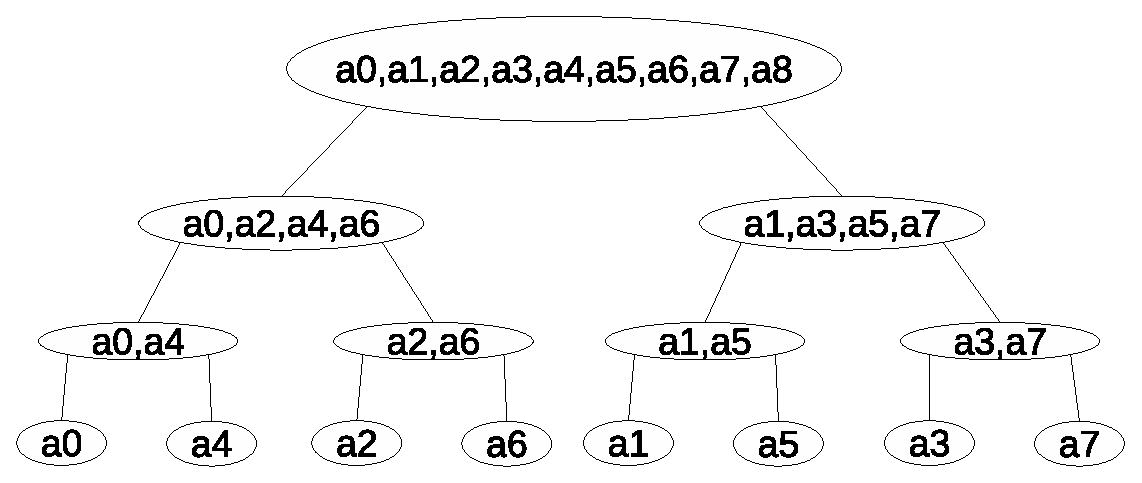
\includegraphics[scale=0.5]{img/recursive_fft_execution.eps}
\caption{Execution path of the recursive FFT algorithm given an input vector a with 8 entries}
\end{figure}

If the 8-element vector above is taken as an example, the desired order is (0,4,2,6,1,5,3,7). In binary, the original input \texttt{(000,001,010,011,100,101,110,111)} becomes \texttt{(000,100,010,110,001,101,011,111)}. A bit-reversal will accomplish this transformation, e.g. for an array index with $d$ bits,
\[
k = b_{d-1}b_{d-2}b_{d-3}...b_0 \rightarrow b_0b_1...b_{d-2}b_{d-1} = k'
\]

The \texttt{Bit-Reverse()} function performs the reordering by:
\begin{lstlisting}
Bit-Reverse(x)
    y = empty vector
    for k in 0..x.length-1
        k2 = reverse_bits(k)
        y[k] = x[k2]
    return y
\end{lstlisting}

Therefore \texttt{Bit-Reverse()} is used to unroll the recursive execution and transform it into an iterative one. The iterative algorithm is also $T(n) = \mathcal{O}(n * log(n))$ similar to the recursive algorithm.

A pseudo code implementation of the iterative Tukey-Cooley algorithm is:
\begin{lstlisting}
FFT_ITER(x)
    Bit-Reverse (x)
    N = x.length
    for s in 1..log(N)
        m = 2^s
        wm = exp(-i2*pi/m)
        w = 1
        for j in 0..(m/2-1)
            for k in j..(n-1) by m
                t = w * x[k + m/2]
                u = x[k]
                x[k] = u + t
                x[k + m/2] = u - t
            w = w*wm
    return x
\end{lstlisting}

\subsection{FFT Performance}
The relative performance of the sequential algorithms discussed above are shown in figure \ref{seqTimes}. These include the plain DFT, recursive and iterative Cooley-Tukey FFT, and the numpy FFT function. The plot is logarithmic along both axes. Clearly the DFT performs the worst. Our iterative and recursive implementations are similar, with the iterative algorithm performing about two times better on average. The numpy implementation is far better, performing about 10 times better on average than our recursive implementation. The similar slopes of the three FFT algorithms confirm that they have the same asymptotic complexity, which we know is $\mathcal{O}(N\log N)$.

\begin{figure}[h!]
\centering
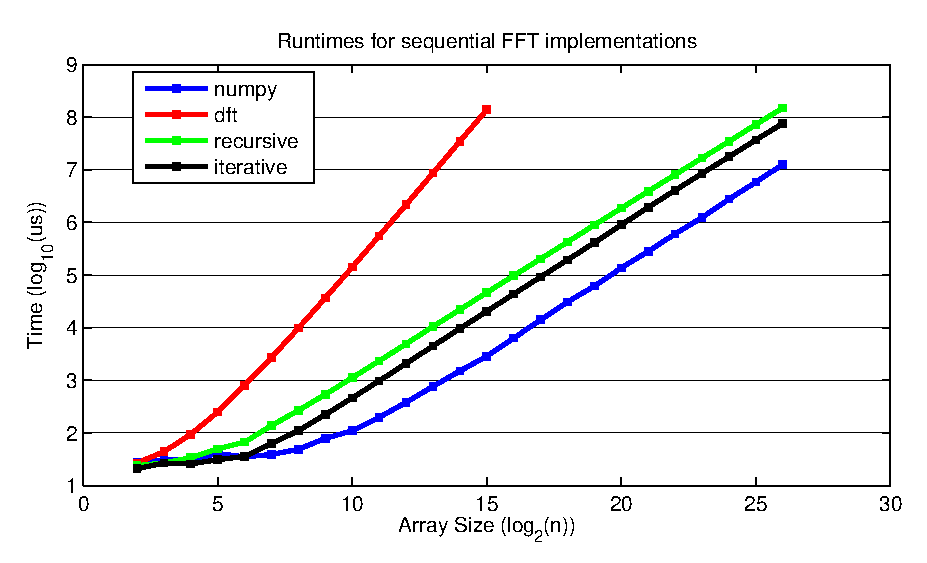
\includegraphics[scale=0.9]{img/seqRuntimes.eps}
\caption{Runtimes for the sequential algorithms.}
\label{seqTimes}
\end{figure}